\begin{figure}[H]
  \centering
  \begin{subfigure}[t]{.48\linewidth}
    \centering
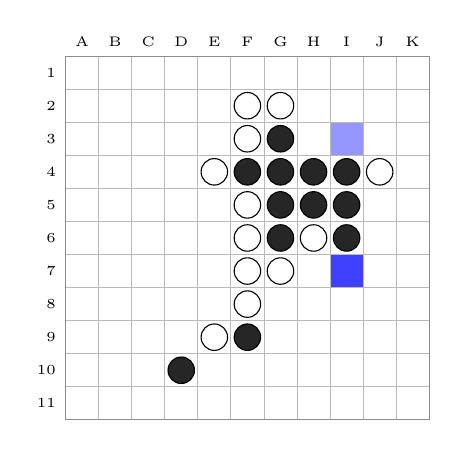
\begin{tikzpicture}[x=0.42cm, y=0.42cm]
\fill[blue!41] (8,-2) rectangle (9,-3);
\fill[blue!75] (8,-6) rectangle (9,-7);
\draw[gray!55, line width=.3pt, step=1] (0,0) grid (11,-11);
\draw[gray!90] (0,0) rectangle (11,-11);
\node[font=\tiny, anchor=south] at (0.5,0) {A};
\node[font=\tiny, anchor=south] at (1.5,0) {B};
\node[font=\tiny, anchor=south] at (2.5,0) {C};
\node[font=\tiny, anchor=south] at (3.5,0) {D};
\node[font=\tiny, anchor=south] at (4.5,0) {E};
\node[font=\tiny, anchor=south] at (5.5,0) {F};
\node[font=\tiny, anchor=south] at (6.5,0) {G};
\node[font=\tiny, anchor=south] at (7.5,0) {H};
\node[font=\tiny, anchor=south] at (8.5,0) {I};
\node[font=\tiny, anchor=south] at (9.5,0) {J};
\node[font=\tiny, anchor=south] at (10.5,0) {K};
\node[font=\tiny, anchor=east] at (0,-0.5) {1};
\node[font=\tiny, anchor=east] at (0,-1.5) {2};
\node[font=\tiny, anchor=east] at (0,-2.5) {3};
\node[font=\tiny, anchor=east] at (0,-3.5) {4};
\node[font=\tiny, anchor=east] at (0,-4.5) {5};
\node[font=\tiny, anchor=east] at (0,-5.5) {6};
\node[font=\tiny, anchor=east] at (0,-6.5) {7};
\node[font=\tiny, anchor=east] at (0,-7.5) {8};
\node[font=\tiny, anchor=east] at (0,-8.5) {9};
\node[font=\tiny, anchor=east] at (0,-9.5) {10};
\node[font=\tiny, anchor=east] at (0,-10.5) {11};
\draw[fill=white, line width=.4pt] (5.5,-1.5) circle (.40);
\draw[fill=white, line width=.4pt] (6.5,-1.5) circle (.40);
\draw[fill=white, line width=.4pt] (5.5,-2.5) circle (.40);
\draw[fill=black!85, line width=.4pt] (6.5,-2.5) circle (.40);
\draw[fill=white, line width=.4pt] (4.5,-3.5) circle (.40);
\draw[fill=black!85, line width=.4pt] (5.5,-3.5) circle (.40);
\draw[fill=black!85, line width=.4pt] (6.5,-3.5) circle (.40);
\draw[fill=black!85, line width=.4pt] (7.5,-3.5) circle (.40);
\draw[fill=black!85, line width=.4pt] (8.5,-3.5) circle (.40);
\draw[fill=white, line width=.4pt] (9.5,-3.5) circle (.40);
\draw[fill=white, line width=.4pt] (5.5,-4.5) circle (.40);
\draw[fill=black!85, line width=.4pt] (6.5,-4.5) circle (.40);
\draw[fill=black!85, line width=.4pt] (7.5,-4.5) circle (.40);
\draw[fill=black!85, line width=.4pt] (8.5,-4.5) circle (.40);
\draw[fill=white, line width=.4pt] (5.5,-5.5) circle (.40);
\draw[fill=black!85, line width=.4pt] (6.5,-5.5) circle (.40);
\draw[fill=white, line width=.4pt] (7.5,-5.5) circle (.40);
\draw[fill=black!85, line width=.4pt] (8.5,-5.5) circle (.40);
\draw[fill=white, line width=.4pt] (5.5,-6.5) circle (.40);
\draw[fill=white, line width=.4pt] (6.5,-6.5) circle (.40);
\draw[fill=white, line width=.4pt] (5.5,-7.5) circle (.40);
\draw[fill=white, line width=.4pt] (4.5,-8.5) circle (.40);
\draw[fill=black!85, line width=.4pt] (5.5,-8.5) circle (.40);
\draw[fill=black!85, line width=.4pt] (3.5,-9.5) circle (.40);
\end{tikzpicture}
    \caption{SL v3: $v=0{,}99$; đáp án 99,9\%; cao nhất I7 (64,1\%)}
  \end{subfigure}\hfill
  \begin{subfigure}[t]{.48\linewidth}
    \centering
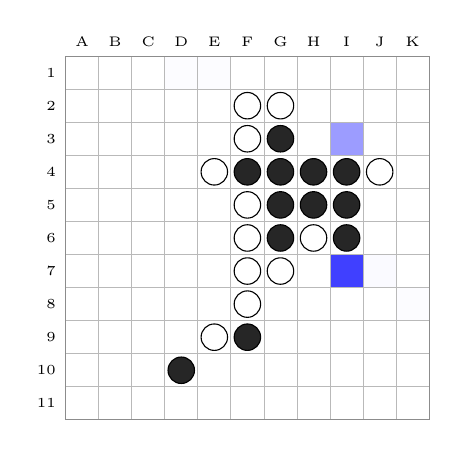
\begin{tikzpicture}[x=0.42cm, y=0.42cm]
\fill[blue!1] (3,0) rectangle (4,-1);
\fill[blue!1] (4,0) rectangle (5,-1);
\fill[blue!39] (8,-2) rectangle (9,-3);
\fill[blue!75] (8,-6) rectangle (9,-7);
\fill[blue!2] (9,-6) rectangle (10,-7);
\fill[blue!1] (10,-7) rectangle (11,-8);
\draw[gray!55, line width=.3pt, step=1] (0,0) grid (11,-11);
\draw[gray!90] (0,0) rectangle (11,-11);
\node[font=\tiny, anchor=south] at (0.5,0) {A};
\node[font=\tiny, anchor=south] at (1.5,0) {B};
\node[font=\tiny, anchor=south] at (2.5,0) {C};
\node[font=\tiny, anchor=south] at (3.5,0) {D};
\node[font=\tiny, anchor=south] at (4.5,0) {E};
\node[font=\tiny, anchor=south] at (5.5,0) {F};
\node[font=\tiny, anchor=south] at (6.5,0) {G};
\node[font=\tiny, anchor=south] at (7.5,0) {H};
\node[font=\tiny, anchor=south] at (8.5,0) {I};
\node[font=\tiny, anchor=south] at (9.5,0) {J};
\node[font=\tiny, anchor=south] at (10.5,0) {K};
\node[font=\tiny, anchor=east] at (0,-0.5) {1};
\node[font=\tiny, anchor=east] at (0,-1.5) {2};
\node[font=\tiny, anchor=east] at (0,-2.5) {3};
\node[font=\tiny, anchor=east] at (0,-3.5) {4};
\node[font=\tiny, anchor=east] at (0,-4.5) {5};
\node[font=\tiny, anchor=east] at (0,-5.5) {6};
\node[font=\tiny, anchor=east] at (0,-6.5) {7};
\node[font=\tiny, anchor=east] at (0,-7.5) {8};
\node[font=\tiny, anchor=east] at (0,-8.5) {9};
\node[font=\tiny, anchor=east] at (0,-9.5) {10};
\node[font=\tiny, anchor=east] at (0,-10.5) {11};
\draw[fill=white, line width=.4pt] (5.5,-1.5) circle (.40);
\draw[fill=white, line width=.4pt] (6.5,-1.5) circle (.40);
\draw[fill=white, line width=.4pt] (5.5,-2.5) circle (.40);
\draw[fill=black!85, line width=.4pt] (6.5,-2.5) circle (.40);
\draw[fill=white, line width=.4pt] (4.5,-3.5) circle (.40);
\draw[fill=black!85, line width=.4pt] (5.5,-3.5) circle (.40);
\draw[fill=black!85, line width=.4pt] (6.5,-3.5) circle (.40);
\draw[fill=black!85, line width=.4pt] (7.5,-3.5) circle (.40);
\draw[fill=black!85, line width=.4pt] (8.5,-3.5) circle (.40);
\draw[fill=white, line width=.4pt] (9.5,-3.5) circle (.40);
\draw[fill=white, line width=.4pt] (5.5,-4.5) circle (.40);
\draw[fill=black!85, line width=.4pt] (6.5,-4.5) circle (.40);
\draw[fill=black!85, line width=.4pt] (7.5,-4.5) circle (.40);
\draw[fill=black!85, line width=.4pt] (8.5,-4.5) circle (.40);
\draw[fill=white, line width=.4pt] (5.5,-5.5) circle (.40);
\draw[fill=black!85, line width=.4pt] (6.5,-5.5) circle (.40);
\draw[fill=white, line width=.4pt] (7.5,-5.5) circle (.40);
\draw[fill=black!85, line width=.4pt] (8.5,-5.5) circle (.40);
\draw[fill=white, line width=.4pt] (5.5,-6.5) circle (.40);
\draw[fill=white, line width=.4pt] (6.5,-6.5) circle (.40);
\draw[fill=white, line width=.4pt] (5.5,-7.5) circle (.40);
\draw[fill=white, line width=.4pt] (4.5,-8.5) circle (.40);
\draw[fill=black!85, line width=.4pt] (5.5,-8.5) circle (.40);
\draw[fill=black!85, line width=.4pt] (3.5,-9.5) circle (.40);
\end{tikzpicture}
    \caption{SL không aug: $v=0{,}97$; đáp án 96,8\%; cao nhất I7 (60,6\%)}
  \end{subfigure}\par\medskip
  \begin{subfigure}[t]{.48\linewidth}
    \centering
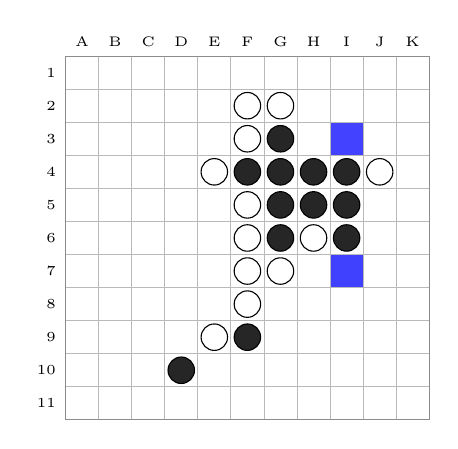
\begin{tikzpicture}[x=0.42cm, y=0.42cm]
\fill[blue!74] (8,-2) rectangle (9,-3);
\fill[blue!75] (8,-6) rectangle (9,-7);
\draw[gray!55, line width=.3pt, step=1] (0,0) grid (11,-11);
\draw[gray!90] (0,0) rectangle (11,-11);
\node[font=\tiny, anchor=south] at (0.5,0) {A};
\node[font=\tiny, anchor=south] at (1.5,0) {B};
\node[font=\tiny, anchor=south] at (2.5,0) {C};
\node[font=\tiny, anchor=south] at (3.5,0) {D};
\node[font=\tiny, anchor=south] at (4.5,0) {E};
\node[font=\tiny, anchor=south] at (5.5,0) {F};
\node[font=\tiny, anchor=south] at (6.5,0) {G};
\node[font=\tiny, anchor=south] at (7.5,0) {H};
\node[font=\tiny, anchor=south] at (8.5,0) {I};
\node[font=\tiny, anchor=south] at (9.5,0) {J};
\node[font=\tiny, anchor=south] at (10.5,0) {K};
\node[font=\tiny, anchor=east] at (0,-0.5) {1};
\node[font=\tiny, anchor=east] at (0,-1.5) {2};
\node[font=\tiny, anchor=east] at (0,-2.5) {3};
\node[font=\tiny, anchor=east] at (0,-3.5) {4};
\node[font=\tiny, anchor=east] at (0,-4.5) {5};
\node[font=\tiny, anchor=east] at (0,-5.5) {6};
\node[font=\tiny, anchor=east] at (0,-6.5) {7};
\node[font=\tiny, anchor=east] at (0,-7.5) {8};
\node[font=\tiny, anchor=east] at (0,-8.5) {9};
\node[font=\tiny, anchor=east] at (0,-9.5) {10};
\node[font=\tiny, anchor=east] at (0,-10.5) {11};
\draw[fill=white, line width=.4pt] (5.5,-1.5) circle (.40);
\draw[fill=white, line width=.4pt] (6.5,-1.5) circle (.40);
\draw[fill=white, line width=.4pt] (5.5,-2.5) circle (.40);
\draw[fill=black!85, line width=.4pt] (6.5,-2.5) circle (.40);
\draw[fill=white, line width=.4pt] (4.5,-3.5) circle (.40);
\draw[fill=black!85, line width=.4pt] (5.5,-3.5) circle (.40);
\draw[fill=black!85, line width=.4pt] (6.5,-3.5) circle (.40);
\draw[fill=black!85, line width=.4pt] (7.5,-3.5) circle (.40);
\draw[fill=black!85, line width=.4pt] (8.5,-3.5) circle (.40);
\draw[fill=white, line width=.4pt] (9.5,-3.5) circle (.40);
\draw[fill=white, line width=.4pt] (5.5,-4.5) circle (.40);
\draw[fill=black!85, line width=.4pt] (6.5,-4.5) circle (.40);
\draw[fill=black!85, line width=.4pt] (7.5,-4.5) circle (.40);
\draw[fill=black!85, line width=.4pt] (8.5,-4.5) circle (.40);
\draw[fill=white, line width=.4pt] (5.5,-5.5) circle (.40);
\draw[fill=black!85, line width=.4pt] (6.5,-5.5) circle (.40);
\draw[fill=white, line width=.4pt] (7.5,-5.5) circle (.40);
\draw[fill=black!85, line width=.4pt] (8.5,-5.5) circle (.40);
\draw[fill=white, line width=.4pt] (5.5,-6.5) circle (.40);
\draw[fill=white, line width=.4pt] (6.5,-6.5) circle (.40);
\draw[fill=white, line width=.4pt] (5.5,-7.5) circle (.40);
\draw[fill=white, line width=.4pt] (4.5,-8.5) circle (.40);
\draw[fill=black!85, line width=.4pt] (5.5,-8.5) circle (.40);
\draw[fill=black!85, line width=.4pt] (3.5,-9.5) circle (.40);
\end{tikzpicture}
    \caption{L6 (RL): $v=0{,}84$; đáp án 100,0\%; cao nhất I7 (50,2\%)}
  \end{subfigure}\hfill
  \begin{subfigure}[t]{.48\linewidth}
    \centering
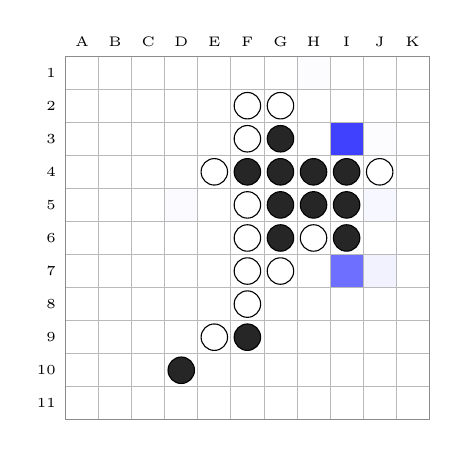
\begin{tikzpicture}[x=0.42cm, y=0.42cm]
\fill[blue!1] (7,0) rectangle (8,-1);
\fill[blue!75] (8,-2) rectangle (9,-3);
\fill[blue!1] (9,-2) rectangle (10,-3);
\fill[blue!2] (3,-4) rectangle (4,-5);
\fill[blue!3] (9,-4) rectangle (10,-5);
\fill[blue!57] (8,-6) rectangle (9,-7);
\fill[blue!5] (9,-6) rectangle (10,-7);
\draw[gray!55, line width=.3pt, step=1] (0,0) grid (11,-11);
\draw[gray!90] (0,0) rectangle (11,-11);
\node[font=\tiny, anchor=south] at (0.5,0) {A};
\node[font=\tiny, anchor=south] at (1.5,0) {B};
\node[font=\tiny, anchor=south] at (2.5,0) {C};
\node[font=\tiny, anchor=south] at (3.5,0) {D};
\node[font=\tiny, anchor=south] at (4.5,0) {E};
\node[font=\tiny, anchor=south] at (5.5,0) {F};
\node[font=\tiny, anchor=south] at (6.5,0) {G};
\node[font=\tiny, anchor=south] at (7.5,0) {H};
\node[font=\tiny, anchor=south] at (8.5,0) {I};
\node[font=\tiny, anchor=south] at (9.5,0) {J};
\node[font=\tiny, anchor=south] at (10.5,0) {K};
\node[font=\tiny, anchor=east] at (0,-0.5) {1};
\node[font=\tiny, anchor=east] at (0,-1.5) {2};
\node[font=\tiny, anchor=east] at (0,-2.5) {3};
\node[font=\tiny, anchor=east] at (0,-3.5) {4};
\node[font=\tiny, anchor=east] at (0,-4.5) {5};
\node[font=\tiny, anchor=east] at (0,-5.5) {6};
\node[font=\tiny, anchor=east] at (0,-6.5) {7};
\node[font=\tiny, anchor=east] at (0,-7.5) {8};
\node[font=\tiny, anchor=east] at (0,-8.5) {9};
\node[font=\tiny, anchor=east] at (0,-9.5) {10};
\node[font=\tiny, anchor=east] at (0,-10.5) {11};
\draw[fill=white, line width=.4pt] (5.5,-1.5) circle (.40);
\draw[fill=white, line width=.4pt] (6.5,-1.5) circle (.40);
\draw[fill=white, line width=.4pt] (5.5,-2.5) circle (.40);
\draw[fill=black!85, line width=.4pt] (6.5,-2.5) circle (.40);
\draw[fill=white, line width=.4pt] (4.5,-3.5) circle (.40);
\draw[fill=black!85, line width=.4pt] (5.5,-3.5) circle (.40);
\draw[fill=black!85, line width=.4pt] (6.5,-3.5) circle (.40);
\draw[fill=black!85, line width=.4pt] (7.5,-3.5) circle (.40);
\draw[fill=black!85, line width=.4pt] (8.5,-3.5) circle (.40);
\draw[fill=white, line width=.4pt] (9.5,-3.5) circle (.40);
\draw[fill=white, line width=.4pt] (5.5,-4.5) circle (.40);
\draw[fill=black!85, line width=.4pt] (6.5,-4.5) circle (.40);
\draw[fill=black!85, line width=.4pt] (7.5,-4.5) circle (.40);
\draw[fill=black!85, line width=.4pt] (8.5,-4.5) circle (.40);
\draw[fill=white, line width=.4pt] (5.5,-5.5) circle (.40);
\draw[fill=black!85, line width=.4pt] (6.5,-5.5) circle (.40);
\draw[fill=white, line width=.4pt] (7.5,-5.5) circle (.40);
\draw[fill=black!85, line width=.4pt] (8.5,-5.5) circle (.40);
\draw[fill=white, line width=.4pt] (5.5,-6.5) circle (.40);
\draw[fill=white, line width=.4pt] (6.5,-6.5) circle (.40);
\draw[fill=white, line width=.4pt] (5.5,-7.5) circle (.40);
\draw[fill=white, line width=.4pt] (4.5,-8.5) circle (.40);
\draw[fill=black!85, line width=.4pt] (5.5,-8.5) circle (.40);
\draw[fill=black!85, line width=.4pt] (3.5,-9.5) circle (.40);
\end{tikzpicture}
    \caption{L8 (AZ): $v=0{,}98$; đáp án 96,4\%; cao nhất I3 (50,6\%)}
  \end{subfigure}\par\medskip
  \caption{Policy của bốn mạng tại thế C3-001 (X đi). Ô càng đậm xác suất càng cao (chuẩn hoá theo ô lớn nhất của từng mạng). Đáp án: I2, K2, I3, J3, J5, K5.}
  \label{fig:cs-policy-c3}
\end{figure}
